%=============================================================================
%  SolveBench -- Final Presentation
%  CSE 402 Project -- Section A2
%  Compile with pdflatex (from inside the Presentation/ folder)
%=============================================================================
\documentclass[aspectratio=169,10pt]{beamer}

\usepackage[utf8]{inputenc}
\usepackage[T1]{fontenc}
\usepackage{lmodern}
\usepackage[scaled=0.92]{helvet}
\renewcommand{\familydefault}{\sfdefault}
\usepackage{amsmath,amssymb}
\usepackage{booktabs}
\usepackage{array}
\usepackage{colortbl}
\usepackage{graphicx}
\usepackage{pifont}
\usepackage{tikz}
\usetikzlibrary{arrows.meta,positioning,shapes.geometric,calc,fit,backgrounds}

%------------------------------------------------ figures live in results/figures/
\graphicspath{{../results/figures/}}

%------------------------------------------------ EDIT ME: group details
\newcommand{\memberOne}{2105037}
\newcommand{\memberTwo}{2105038}
\newcommand{\memberThree}{2105042}
\newcommand{\memberFour}{2105047}
\newcommand{\memberFive}{2105054}

%------------------------------------------------ palette (same as linear.tex)
\definecolor{LSnavy}{RGB}{15,52,80}
\definecolor{LSteal}{RGB}{18,110,120}
\definecolor{LSgold}{RGB}{193,138,52}
\definecolor{LSgreen}{RGB}{40,120,86}
\definecolor{LSred}{RGB}{176,58,58}
\definecolor{LSbg}{RGB}{252,251,248}
\definecolor{LSgray}{RGB}{92,100,108}
\definecolor{LSlight}{RGB}{234,240,240}
\definecolor{LSlightgold}{RGB}{247,241,229}

%------------------------------------------------ beamer look & feel
\usetheme{default}
\setbeamertemplate{navigation symbols}{}
\setbeamercolor{background canvas}{bg=LSbg}
\setbeamercolor{normal text}{fg=LSnavy}
\setbeamercolor{structure}{fg=LSteal}
\setbeamercolor{frametitle}{fg=LSnavy,bg=LSbg}
\setbeamercolor{title}{fg=LSnavy}
\setbeamercolor{itemize item}{fg=LSteal}
\setbeamercolor{itemize subitem}{fg=LSgold}
\setbeamercolor{block title}{fg=white,bg=LSteal}
\setbeamercolor{block body}{fg=LSnavy,bg=LSlight}

% never break a word with a hyphen in a title or a wide bold line -- it reads as
% unpolished on a slide, where the fix is always to reword rather than to hyphenate
\hyphenpenalty=10000
\exhyphenpenalty=10000

\setbeamerfont{frametitle}{series=\bfseries,size=\large}
\setbeamerfont{title}{series=\bfseries,size=\Large}
\setbeamerfont{block title}{series=\bfseries}
\setbeamertemplate{itemize item}{\small\raise0.15ex\hbox{\ding{110}}}
\setbeamertemplate{itemize subitem}{\footnotesize\raise0.1ex\hbox{\ding{119}}}

\setbeamertemplate{frametitle}{%
  \vspace{0.55em}%
  \begin{beamercolorbox}[wd=\paperwidth,leftskip=0.9cm,rightskip=0.9cm]{frametitle}%
    \strut\insertframetitle\strut\par
    {\color{LSteal}\rule{0.55\linewidth}{1.4pt}}%
    {\color{LSgold}\rule{0.10\linewidth}{1.4pt}}%
  \end{beamercolorbox}%
}

\setbeamertemplate{footline}{%
  \hbox{%
    \begin{beamercolorbox}[wd=.36\paperwidth,ht=2.4ex,dp=1.1ex,leftskip=0.9cm]{}%
      {\color{LSgray}\scriptsize SolveBench}\hfill%
    \end{beamercolorbox}%
    \begin{beamercolorbox}[wd=.44\paperwidth,ht=2.4ex,dp=1.1ex,center]{}%
      {\color{LSgray}\scriptsize CSE 402 Final Presentation}%
    \end{beamercolorbox}%
    \begin{beamercolorbox}[wd=.20\paperwidth,ht=2.4ex,dp=1.1ex,rightskip=0.9cm]{}%
      \hfill{\color{LSteal}\scriptsize\bfseries\insertframenumber}%
    \end{beamercolorbox}%
  }\vspace{1pt}%
}

%------------------------------------------------ macros
\renewcommand{\emph}[1]{{\color{LSteal}\bfseries #1}}
\newcommand{\gd}[1]{{\color{LSgreen}\bfseries #1}}
\newcommand{\bad}[1]{{\color{LSred}\bfseries #1}}
\newcommand{\hdrow}{\rowcolor{LSnavy}}
\newcommand{\hdtxt}[1]{\textcolor{white}{\bfseries #1}}
\newcommand{\subtag}[1]{\\{\scriptsize\color{LSgray}\normalfont #1}}

% shared tikz styles for flow diagrams
\tikzset{
  stage/.style={rounded corners=3pt,draw=LSteal,line width=1pt,fill=LSlight,
                text=LSnavy,align=center,inner sep=6pt,font=\footnotesize\bfseries},
  data/.style={rounded corners=3pt,draw=LSgold,line width=1pt,fill=LSlightgold,
               text=LSnavy,align=center,inner sep=6pt,font=\footnotesize},
  outbox/.style={rounded corners=3pt,draw=LSgreen,line width=1.2pt,fill=LSlightgold,
               text=LSnavy,align=center,inner sep=6pt,font=\footnotesize\bfseries},
  fl/.style={-{Stealth[length=2.6mm]},line width=1.1pt,draw=LSteal},
}

% a full-bleed navy divider slide, used between the seven parts of the story
\newcommand{\dividerframe}[3]{%
\begin{frame}[plain]
  \begin{tikzpicture}[remember picture,overlay]
    \fill[LSnavy] (current page.north west) rectangle (current page.south east);
    \fill[LSgold] ([yshift=0.0cm,xshift=0.9cm]current page.south west) rectangle
                  ([yshift=0.14cm,xshift=2.6cm]current page.south west);
  \end{tikzpicture}
  \vspace{2.5cm}
  \hspace{0.9cm}%
  \begin{minipage}{0.82\linewidth}
    {\color{LSgold}\bfseries\large #1}\\[0.5em]
    {\color{white}\fontsize{27}{31}\selectfont\bfseries #2}\\[0.7em]
    {\color{LSlight}\normalsize #3}
  \end{minipage}
\end{frame}}

% a large centred "hero number" slide for the two or three statistics that carry
% the whole story on their own
\newcommand{\heroframe}[3]{%
\begin{frame}[plain]{#1}
  \vspace{0.4cm}
  \begin{center}
  {\color{LSnavy}\fontsize{58}{60}\selectfont\bfseries #2}\\[0.5em]
  {\color{LSgray}\large #3}
  \end{center}
\end{frame}}

% consistent, safe figure inclusion: capped by BOTH width and height, so a figure
% can never run past either edge of the slide regardless of its own aspect ratio
\newcommand{\slidefig}[2][0.94]{%
  \includegraphics[width=#1\textwidth,height=0.66\textheight,keepaspectratio]{#2}}
\newcommand{\slidefigtall}[2][0.94]{%
  \includegraphics[width=#1\textwidth,height=0.76\textheight,keepaspectratio]{#2}}
\newcommand{\halffig}[1]{%
  \includegraphics[width=\linewidth,height=0.56\textheight,keepaspectratio]{#1}}

%=============================================================================
\title{SolveBench}
\subtitle{Direct and Iterative Linear Solvers on Real Engineering Data}
\date{}
%=============================================================================
\begin{document}

%----------------------------------------------------------------- TITLE
\begin{frame}[plain]
  \begin{tikzpicture}[remember picture,overlay]
    \fill[LSnavy] (current page.south west) rectangle ([yshift=2.0cm]current page.south east);
    \node[anchor=west] at ([yshift=1.0cm,xshift=0.9cm]current page.south west)
      {\color{LSgold}\footnotesize\bfseries Section A2 $\cdot$ Roll Numbers \;\;
       \color{LSlight}\normalfont \memberOne\ $\cdot$ \memberTwo\ $\cdot$ \memberThree\ $\cdot$ \memberFour\ $\cdot$ \memberFive};
    \fill[LSgold] ([yshift=7.86cm,xshift=0.92cm]current page.south west) rectangle
                  ([yshift=7.72cm,xshift=2.5cm]current page.south west);
  \end{tikzpicture}
  \vspace{0.9cm}
  \hspace{0.4cm}%
  \begin{minipage}{0.94\linewidth}
    {\color{LSteal}\bfseries\large SOLVEBENCH}\\[0.45em]
    {\color{LSnavy}\fontsize{27}{31}\selectfont\bfseries Solving $A\vec{x}=\vec{b}$ at Scale}\\[0.3em]
    {\color{LSnavy}\Large A Diagonal-Selection Pipeline for Stationary Iterative Solvers}\\[0.85em]
    {\color{LSgray}\normalsize Every blackout-prevention study and every bridge safety check
     reduces to this exact equation. We benchmarked 16 solvers on 927 real matrices,
     found what breaks, and built a fix for it.}
  \end{minipage}
\end{frame}

%----------------------------------------------------------------- AGENDA
\begin{frame}{Where This Talk Is Going}
  \small
  \vspace{0.2em}
  This is the full story, in the order it actually happened. Seven parts.
  \vspace{0.5em}
  \begin{columns}[T]
    \begin{column}{0.49\textwidth}
      \begin{enumerate}\setlength\itemsep{0.45em}
        \item \textbf{\color{LSteal}The problem} we are solving, and the paper we extend
        \item \textbf{\color{LSteal}What we implemented} from that paper
        \item \textbf{\color{LSteal}Scaling the experiment} from 5 unknowns to 927 real matrices
        \item \textbf{\color{LSteal}Baseline results} across all 16 solvers
      \end{enumerate}
    \end{column}
    \begin{column}{0.49\textwidth}
      \begin{enumerate}\setlength\itemsep{0.45em}\setcounter{enumi}{4}
        \item \textbf{\color{LSteal}The story of our novelty}, milestone by milestone,
          starting from our first idea (APK)
        \item \textbf{\color{LSteal}Honest limits}: what we do not claim
        \item \textbf{\color{LSteal}Where things stand}, and what is next
      \end{enumerate}
    \end{column}
  \end{columns}
  \vspace{0.7em}
  \begin{center}
  \colorbox{LSlightgold}{\parbox{0.9\linewidth}{\centering\footnotesize
  Every number in this deck is measured and traceable to a table in the repository.
  Where a result is still being measured, we say so.}}
  \end{center}
\end{frame}

%=============================================================================
\dividerframe{PART 1}{The Problem We Solve}{Why $A\vec{x}=\vec{b}$ is the one equation every simulation eventually hits}
%=============================================================================

\begin{frame}{What Problem Are We Solving?}
  \small
  Almost every engineering simulation, whether it is a power grid, a bridge, a
  circuit, or an airflow model, reduces to the same piece of algebra:
  \begin{center}
  {\LARGE\color{LSnavy}\bfseries $A\vec{x} = \vec{b}$}
  \end{center}
  \vspace{0.3em}
  $A$ is huge and \emph{sparse}: almost every entry is exactly zero, because most
  parts of a physical system only interact with their close neighbours.
  \vspace{0.5em}
  \begin{columns}[T]
    \begin{column}{0.49\textwidth}
      \textbf{\color{LSteal}Direct methods}\\[0.2em]
      \footnotesize Factor $A = LU$, then solve two easy triangular systems.
      Exact answer, fixed number of steps. Can need huge memory for fill-in.
    \end{column}
    \begin{column}{0.49\textwidth}
      \textbf{\color{LSteal}Iterative methods}\\[0.2em]
      \footnotesize Start from a guess, improve it step by step, stop once the
      residual is small. Cheap per step. May never get closer at all.
    \end{column}
  \end{columns}
  \vspace{0.6em}
  \begin{block}{\small The whole project, in one sentence}
    \footnotesize Whether an iterative method converges depends entirely on the
    structure of $A$. That dependency is what this project measures, on real data.
  \end{block}
\end{frame}

\begin{frame}{Base Paper: What It Studies}
  \vspace{-0.15em}
  \colorbox{LSlight}{\parbox{0.98\linewidth}{\vspace{0.2em}
    {\bfseries\normalsize\color{LSnavy} ``Comparative Analysis of Jacobi and Gauss-Seidel Iterative Methods''}\\[0.18em]
    {\footnotesize\color{LSgray} P.\ Khrapov and N.\ Volkov}\\[0.12em]
    {\footnotesize\color{LSteal}\emph{International Journal of Open Information Technologies}, vol.\ 12, no.\ 2, pp.\ 23--34, 2024}
    \vspace{0.2em}}}
  \vspace{0.35em}
  \small
  \begin{itemize}\setlength\itemsep{0.3em}
    \item Works out, by hand, exactly which \textbf{2 and 3 unknown} matrices make
      Jacobi and Gauss-Seidel converge.
    \item Checks that pattern statistically on \textbf{random matrices}, up to 5
      unknowns, generated by computer.
    \item Shows the two methods do \emph{not} always share a convergence region:
      which one wins depends on the matrix.
  \end{itemize}
  \vspace{0.4em}
  \begin{block}{\small The gap this leaves open}
    \footnotesize The paper never once touches a matrix from a real engineering
    problem. Everything is either worked out by hand at toy size, or generated at
    random. Random numbers do not look like real data: they carry none of the
    structure that comes from how a real circuit or bridge is actually built.
  \end{block}
\end{frame}

\begin{frame}{The Gap, and Our Question}
  \small
  \vspace{0.2em}
  Nobody has checked whether the paper's conclusions survive contact with matrices
  that engineers actually have to solve, at the sizes those methods are actually
  used at.
  \vspace{0.6em}
  \begin{center}
  \colorbox{LSlightgold}{\parbox{0.92\linewidth}{\centering\small
  \textbf{Our question:} do Jacobi and Gauss-Seidel behave the way the theory says
  on real engineering matrices, and where do they stand once you put the solvers an
  engineer would actually reach for beside them?}}
  \end{center}
  \vspace{0.7em}
  \small
  This is an \textbf{exploratory and comparative study}: we benchmark direct,
  stationary, Krylov, and preconditioned solvers against 927 real matrices, and we
  build one genuinely new preprocessing idea on top of what we find.
\end{frame}

%=============================================================================
\dividerframe{PART 2}{What We Built From the Paper}{Jacobi, Gauss-Seidel, SOR, and the convergence theory behind them}
%=============================================================================

\begin{frame}{Jacobi and Gauss-Seidel: the Update Rules}
  \small
  Split $A = D + L + U$: the diagonal, everything below it, everything above it.
  \vspace{0.5em}
  \begin{columns}[T]
    \begin{column}{0.49\textwidth}
      \begin{center}\textbf{\color{LSteal}Jacobi}\end{center}
      \vspace{0.2em}
      \[ \vec{x}^{(k+1)} = D^{-1}\left(\vec{b} - (L+U)\vec{x}^{(k)}\right) \]
      \footnotesize Every entry uses only values from the \emph{previous} full pass.
      One matrix-vector product per step.
    \end{column}
    \begin{column}{0.49\textwidth}
      \begin{center}\textbf{\color{LSteal}Gauss-Seidel}\end{center}
      \vspace{0.2em}
      \[ \vec{x}^{(k+1)} = (D+L)^{-1}\left(\vec{b} - U\vec{x}^{(k)}\right) \]
      \footnotesize Each row can use \emph{already-updated} values from earlier
      rows in the same pass. Usually faster than Jacobi.
    \end{column}
  \end{columns}
  \vspace{0.7em}
  \begin{block}{\small Both need one thing to even exist}
    \footnotesize Both divide by the diagonal entries of $D$. If any $a_{ii} = 0$,
    that division is impossible: the method is not slow, it is \bad{undefined}.
  \end{block}
\end{frame}

\begin{frame}{SOR, and Whether Any of This Converges}
  \small
  \textbf{\color{LSteal}SOR (Successive Over-Relaxation)} adds one tuning number,
  $\omega$, that lets the update overshoot on purpose:
  \[ (D+\omega L)\,\vec{\delta} = \omega\,\vec{r}, \qquad \vec{x} \leftarrow \vec{x}+\vec{\delta} \]
  \footnotesize $\omega = 1$ reduces exactly to Gauss-Seidel. The base paper's proposal
  and our own results (Part 5) both use this third method.
  \vspace{0.6em}
  \small
  \textbf{\color{LSteal}Convergence itself is governed by one number}, the spectral
  radius $\rho(T)$ of the method's iteration matrix $T$:
  \[ \rho(T) < 1 \;\Rightarrow\; \text{converges, eventually} \qquad
     \rho(T) \ge 1 \;\Rightarrow\; \text{does not converge} \]
  \footnotesize $\rho(T)$ also sets the speed: reaching tolerance $\varepsilon$ takes
  roughly $\log(\varepsilon)/\log(\rho(T))$ steps. $\rho=0.5$ needs about 27 steps;
  $\rho=0.999$ needs about 18{,}000.
\end{frame}

\begin{frame}{The Full Method Roster: 16 Solvers, 5 Families}
  \small
  We did not stop at the two methods the paper studies. Without a floor and a
  ceiling, ``Jacobi is slow'' is not a meaningful sentence.
  \vspace{0.4em}
  \renewcommand{\arraystretch}{1.28}
  \begin{center}
  \begin{tabular}{@{}p{2.8cm}p{6.9cm}p{1.4cm}@{}}
    \toprule
    \hdrow \hdtxt{Family} & \hdtxt{Methods} & \hdtxt{Count}\\
    \midrule
    Direct, hand-written & Gauss elimination, Gauss-Jordan, LU, Cholesky & 4\\
    \rowcolor{LSlight}
    Direct, library & \texttt{spsolve}, \texttt{splu} (SuperLU) & 2\\
    \textbf{Stationary} & \textbf{Jacobi, Gauss-Seidel, SOR} & \textbf{3}\\
    \rowcolor{LSlight}
    Krylov & Conjugate Gradient, BiCGSTAB, GMRES(30) & 3\\
    Preconditioned & ILU only, ILU-BiCGSTAB, ILU-GMRES(30), ILU-Krylov (dispatched) & 4\\
    \bottomrule
  \end{tabular}
  \end{center}
  \vspace{0.5em}
  \footnotesize\color{LSgray}
  The last row, ILU-Krylov (dispatched), is our original course proposal, APK. Its
  story is told honestly in Part 5.
\end{frame}

%=============================================================================
\dividerframe{PART 3}{Scaling the Experiment Up}{From 5 unknowns and random numbers to 927 real matrices at $n \le 10{,}000$}
%=============================================================================

\begin{frame}{How Much We Scaled It Up}
  \small
  \renewcommand{\arraystretch}{1.3}
  \begin{center}
  \begin{tabular}{@{}p{3.4cm}p{4.1cm}p{4.1cm}@{}}
    \toprule
    \hdrow \hdtxt{} & \hdtxt{The paper} & \hdtxt{This project}\\
    \midrule
    Matrix source & hand-derived, then random & real engineering data\\
    \rowcolor{LSlight}
    Matrix count & a handful, then a random batch & \textbf{927 unique matrices}\\
    Matrix size & up to 5 unknowns & \textbf{up to 10{,}000 unknowns}\\
    \rowcolor{LSlight}
    Domains & none (random numbers) & \textbf{26 real domains}\\
    Methods compared & Jacobi, Gauss-Seidel & \textbf{16 methods, 5 families}\\
    \bottomrule
  \end{tabular}
  \end{center}
  \vspace{0.6em}
  \footnotesize\color{LSgray}
  Source: the SuiteSparse Matrix Collection, the standard public library of real
  sparse matrices contributed by engineers from actual projects.
\end{frame}

\begin{frame}{26 Domains, 927 Matrices}
  \begin{center}
  \slidefig[0.62]{22_domain_composition.png}
  \end{center}
  \vspace{0.2em}
  \footnotesize\color{LSgray}\centering
  One domain has 200 matrices, eight have fewer than 5. Every per-domain claim in
  this project reports its own $n$ for exactly this reason.
\end{frame}

\begin{frame}{What the Matrices Actually Look Like}
  \begin{center}
  \slidefig[0.98]{18_matrix_gallery.png}
  \end{center}
  \vspace{0.3em}
  \footnotesize\color{LSgray}\centering
  A spy plot: one dot per nonzero entry, position only. A circuit, a structural
  mesh, a 2D/3D problem and a fluid-dynamics discretisation do not just differ in
  numbers, they differ in shape.
\end{frame}

\begin{frame}{Corpus Bookkeeping: Being Honest About 930 Files}
  \small
  \vspace{0.2em}
  \begin{itemize}\setlength\itemsep{0.5em}
    \item 930 files downloaded. \textbf{3 are exact duplicates} of other files under
      a different name $\Rightarrow$ \textbf{927 unique matrices}.
    \item \textbf{6 files were truncated downloads}: each file's own header declared
      more nonzero entries than the file contained, so they silently failed to
      load. Usable corpus: \textbf{924}.
    \item \textbf{100 of the 930 are random matrices we generated ourselves}, sizes
      5 to 300, specifically to reproduce the base paper's own validation method
      (Part 4 shows what that comparison found).
    \item One domain was spelled two ways in the source data, splitting it in two
      by accident. We merge it back.
  \end{itemize}
  \vspace{0.5em}
  \begin{block}{\small Why this matters}
    \footnotesize A downloaded file that is never checked against its own declared
    size can silently break a result months later. This is one of the mistakes we
    made and fixed (Part 5, and the closing section).
  \end{block}
\end{frame}

\begin{frame}{How We Decide a Solve Actually Succeeded}
  \small
  \vspace{0.1em}
  A solver's own claim of success is \bad{recorded, never trusted}. Success is
  decided afterwards, by us, from the residual we measure independently:
  \[ \text{relative residual} = \|A\vec{x}-\vec{b}\| / \|\vec{b}\| \le 10^{-8} \;\Rightarrow\; \text{solved} \]
  \vspace{0.3em}
  \footnotesize
  \begin{columns}[T]
    \begin{column}{0.49\textwidth}
      \begin{itemize}\setlength\itemsep{0.2em}\footnotesize
        \item \gd{solved}: residual verified below tolerance
        \item \bad{inaccurate}: solver claimed success, residual disagrees
        \item did\_not\_converge: solver admitted failure
        \item diverged: the iterate blew up
      \end{itemize}
    \end{column}
    \begin{column}{0.49\textwidth}
      \begin{itemize}\setlength\itemsep{0.2em}\footnotesize
        \item not\_applicable: undefined on this matrix
        \item structurally\_singular: no unique solution
        \item skipped\_too\_large: deliberately not attempted
        \item error: an unexpected failure, recorded
      \end{itemize}
    \end{column}
  \end{columns}
  \vspace{0.4em}
  \colorbox{LSlightgold}{\parbox{0.96\linewidth}{\footnotesize
  The very first version of this project trusted a solver's own success flag, and
  passed 57 solves whose actual residual reached $9.71\times10^{12}$.}}
\end{frame}

%=============================================================================
\dividerframe{PART 4}{Baseline Results Across All 16 Solvers}{What each method can actually do on 927 real matrices}
%=============================================================================

\begin{frame}{Applicability vs.\ Conditional Success, All 16 Methods}
  \begin{center}
  \slidefig[0.78]{04_method_scoreboard.png}
  \end{center}
  \footnotesize\color{LSgray}\centering
  Two rates, never multiplied. Conjugate Gradient is applicable on only 11.7\% of
  the corpus, but solves 84.3\% of what it is allowed to try.
\end{frame}

\begin{frame}{The Full Numbers, Ranked by Systems Solved}
  \scriptsize
  \renewcommand{\arraystretch}{1.18}
  \begin{center}
  \begin{tabular}{@{}p{4.3cm}p{1.5cm}p{1.3cm}p{1.7cm}p{1.9cm}@{}}
    \toprule
    \hdrow \hdtxt{Method} & \hdtxt{Applic.} & \hdtxt{Solved} & \hdtxt{Applicability} & \hdtxt{Cond.\ success}\\
    \midrule
    \texttt{spsolve} (SuperLU) & 901 & \gd{874} & 97.2\% & 97.0\%\\
    \rowcolor{LSlight}
    \texttt{splu} (SuperLU) & 885 & 874 & 95.5\% & 98.8\%\\
    ILU-Krylov (dispatched) & 736 & 617 & 79.4\% & 83.8\%\\
    \rowcolor{LSlight}
    Gauss elimination / LU & 596 & 593 & 64.3\% & 99.5\%\\
    BiCGSTAB & 902 & 341 & 97.3\% & 37.8\%\\
    \rowcolor{LSlight}
    Gauss-Seidel & 411 & 121 & 44.3\% & 29.4\%\\
    Conjugate Gradient & 108 & 91 & 11.7\% & 84.3\%\\
    \rowcolor{LSlight}
    Jacobi & 411 & 75 & 44.3\% & 18.2\%\\
    \bottomrule
  \end{tabular}
  \end{center}
  \vspace{0.4em}
  \footnotesize\color{LSgray}\centering
  All 16 rows, with every denominator, are in \texttt{RESULTS.md}.
\end{frame}

\begin{frame}{Speed and Robustness, in One Picture}
  \begin{center}
  \slidefig[0.82]{05_performance_profile.png}
  \end{center}
  \footnotesize\color{LSgray}\centering
  A Dolan-Moré performance profile, the standard tool for comparing solvers. Height
  at $\tau{=}1$: how often a method is outright fastest. The right-hand plateau: how
  much of the corpus it can solve at all.
\end{frame}

\begin{frame}{Cost and Iteration Count}
  \begin{columns}[T]
    \begin{column}{0.49\textwidth}
      \centering\halffig{08_cost_profile.png}
    \end{column}
    \begin{column}{0.49\textwidth}
      \centering\halffig{10_iteration_counts.png}
    \end{column}
  \end{columns}
  \vspace{0.3em}
  \footnotesize\color{LSgray}\centering
  Cost is counted in matrix-vector products, not seconds: shared Kaggle hardware
  makes wall-clock time unreproducible. One preconditioned step costs far more
  arithmetic than one Jacobi step, so fewer iterations is not the same as less work.
\end{frame}

\begin{frame}{Does the Textbook Theory Predict the Outcome?}
  \begin{columns}[T]
    \begin{column}{0.49\textwidth}
      \centering\halffig{12_hypothesis_coverage.png}
    \end{column}
    \begin{column}{0.49\textwidth}
      \centering\halffig{13_prediction_vs_observation.png}
    \end{column}
  \end{columns}
  \vspace{0.3em}
  \footnotesize\color{LSgray}\centering
  Stein-Rosenberg (1948) and Householder-John (1958) cover part of the corpus.
  ``too\_slow'' is the case the textbook criterion cannot express: $\rho<1$, so
  convergence is guaranteed, but not inside any usable iteration budget.
\end{frame}

\heroframe{The Single Most Important Fact We Found}{491 of 927}{matrices leave Jacobi, Gauss-Seidel and SOR mathematically undefined, all at once, because of one zero on the diagonal}

\begin{frame}{The Base Paper's Own Test Bed, at Real Scale}
  \begin{center}
  \slidefig[0.6]{23_random_matrices.png}
  \end{center}
  \vspace{0.2em}
  \footnotesize\color{LSgray}\centering
  100 random matrices, sizes 5 to 300, exactly the kind the base paper validates its
  theory on. $\rho(T_{Jacobi})$ grows roughly in proportion to size on random
  matrices, so the paper's own method stops working almost as soon as it is scaled
  up even slightly.
\end{frame}

%=============================================================================
\dividerframe{PART 5}{The Story of Our Novelty}{Ten milestones, in the order they actually happened, starting from our first idea}
%=============================================================================

\begin{frame}{Milestone 0: Our Starting Point, APK}
  \small
  Our original proposal: inspect the matrix, then dispatch to the right Krylov
  method.
  \[ \text{symmetric} \Rightarrow \text{PCG}, \qquad \text{otherwise} \Rightarrow \text{BiCGSTAB} \]
  both preconditioned with ILU.
  \vspace{0.4em}
  \begin{block}{\small What we found when we measured it honestly}
    \footnotesize This exact rule already has a name: the dispatch logic in
    Barrett et al., \emph{Templates} (SIAM, 1994), and the default behaviour of
    PETSc and MATLAB's backslash operator. It was not new.
  \end{block}
  \vspace{0.4em}
  \begin{center}
  \colorbox{LSlightgold}{\parbox{0.92\linewidth}{\centering\small
  ILU-Krylov, dispatched: \textbf{617} of 736 solved.\quad
  Always ILU-BiCGSTAB, no dispatch at all: \textbf{616}.\\[0.2em]
  \bad{One matrix, out of 736.}}}
  \end{center}
  \vspace{0.3em}
  \footnotesize\color{LSgray}
  Kept today as an honestly labelled baseline, not as our novelty. This is why the
  project needed a real contribution.
\end{frame}

\begin{frame}{Milestone 1--2: an Honest Harness, and the 491}
  \small
  Before any new idea could be tested fairly, the benchmark itself had to be
  trustworthy. We rebuilt it, fixing five separate problems (Part 7 lists all
  eight mistakes found across the whole project).
  \vspace{0.4em}
  Once it could be trusted, the very first full sweep produced the number that
  reshaped everything that followed:
  \vspace{0.3em}
  \begin{center}
  \colorbox{LSlight}{\parbox{0.9\linewidth}{\centering\small
  \textbf{491 of 927 matrices (53\%) have at least one zero on the diagonal.}\\
  Jacobi, Gauss-Seidel and SOR cannot even attempt them.}}
  \end{center}
  \vspace{0.5em}
  \footnotesize
  This turned the question from ``is Jacobi slow?'' into a much bigger one:
  \emph{can we make Jacobi applicable in the first place?}
\end{frame}

\begin{frame}{Milestone 3: the Idea, Choose the Diagonal}
  \small
  Row order is arbitrary. It was decided by the meshing software or the circuit
  numbering convention, never by the solver that will run later. Permuting rows
  changes nothing about the answer:
  \[ A' = PA,\quad \vec{b}' = P\vec{b} \;\Rightarrow\; A'\vec{x} = PA\vec{x} = P\vec{b} = \vec{b}' \]
  \vspace{0.4em}
  \begin{center}
  \colorbox{LSlightgold}{\parbox{0.85\linewidth}{\centering\footnotesize
  $A = \begin{pmatrix}0 & 5\\ 3 & 1\end{pmatrix}$: $a_{11}{=}0$, undefined for every
  stationary method.\\
  Swap the rows: $A' = \begin{pmatrix}3 & 1\\ 0 & 5\end{pmatrix}$, and every method
  can now run. Same equations, same answer.}}
  \end{center}
  \vspace{0.5em}
  \footnotesize
  \textbf{\color{LSteal}This single idea is the seed of everything in the rest of
  this part.}
\end{frame}

\begin{frame}{Milestone 4: Proving What Can and Cannot Work}
  \small
  Before searching for a good row order, we checked what kinds of change could
  possibly help, so the search would not waste time on something pointless.
  \vspace{0.4em}
  \begin{itemize}\setlength\itemsep{0.4em}
    \item \textbf{Row scaling} leaves Jacobi's iteration matrix algebraically
      identical: $T_J' = I - (RD)^{-1}RA = T_J$, exactly.
    \item \textbf{Column scaling} is a similarity transform: never changes the
      spectral radius.
    \item \textbf{Symmetric permutation} barely moved it on real matrices: the
      fifth decimal place, $0.99012 \to 0.99011$.
    \item \textbf{Row permutation alone} is the only operation that changes which
      entries sit on $D$.
  \end{itemize}
  \vspace{0.4em}
  \footnotesize\color{LSgray}
  This proof, not a guess, is why we searched over row permutations specifically.
\end{frame}

\begin{frame}{Milestone 5: the Objective, and a False Start}
  \small
  Choosing the diagonal is an \emph{assignment problem}, solvable exactly.
  \vspace{0.3em}
  \begin{columns}[T]
    \begin{column}{0.49\textwidth}
      \textbf{\color{LSteal}MC64 (established)}\\[0.15em]
      \footnotesize maximise $\prod |a_{ii}|$\\[0.3em]
      Built for pivot stability in \emph{direct} solvers. Never looks at the rest
      of the row.
    \end{column}
    \begin{column}{0.49\textwidth}
      \textbf{\color{LSteal}Bottleneck (ours)}\\[0.15em]
      \footnotesize minimise $\displaystyle\max_i \frac{\sum_{j\ne i}|a_{ij}|}{|a_{ii}|}$\\[0.3em]
      Below 1 for every row \textbf{is} strict diagonal dominance, which
      guarantees convergence.
    \end{column}
  \end{columns}
  \vspace{0.5em}
  \colorbox{LSlightgold}{\parbox{0.96\linewidth}{\footnotesize
  \textbf{The false start:} a second objective, min-sum, was meant as a natural
  contrast. Algebra shows $\sum\log(1{+}\text{ratio}) = \text{const} - \sum\log|a_{ii}|$:
  min-sum \textbf{is} MC64 under another name. Verified on 193 matrices, 193 matches.}}
\end{frame}

\begin{frame}{Milestone 6: Four scipy Hangs}
  \begin{center}
  \slidefig[0.92]{19_hang_fixes.png}
  \end{center}
  \vspace{0.2em}
  \footnotesize\color{LSgray}\centering
  Two ready-made scipy matching routines hung, four separate times, in four
  separate ways, on real matrices. One of them stalled an entire 12.7-hour Kaggle
  session. The fix each time: a dense assignment instead.
\end{frame}

\begin{frame}{Milestone 7: What Reordering Actually Buys}
  \begin{center}
  \slidefig[0.62]{20_incremental_gains.png}
  \end{center}
  \vspace{0.2em}
  \footnotesize\color{LSgray}\centering
  199 systems recovered, zero lost. But 195 of the 199 are recovered by \emph{both}
  objectives: the idea of reordering is the large effect, our own choice of
  objective is the small one.
\end{frame}

\begin{frame}{Milestone 7 (continued): Our Objective, Head to Head}
  \begin{center}
  \slidefig[0.75]{03_dominance.png}
  \end{center}
  \footnotesize\color{LSgray}\centering
  On the quantity bottleneck is built to minimise, it beats MC64 \textbf{367 to 0},
  506 ties, never once losing. What that win does not buy: not one further matrix
  in the corpus can be pushed under the diagonal-dominance threshold by any row
  permutation. 43 already were.
\end{frame}

\begin{frame}{Milestone 8: the ILU Hole}
  \begin{center}
  \slidefig[0.86]{02_ilu_hole.png}
  \end{center}
  \vspace{0.2em}
  \footnotesize\color{LSgray}\centering
  166 matrices where no ILU preconditioner could be built at all, taking the whole
  preconditioned family down together. Reordering makes 150 of the 166 buildable,
  and 17 solve outright.
\end{frame}

\begin{frame}{Milestone 9: the Relaxation Factor, Chosen per Matrix}
  \begin{center}
  \slidefig[0.58]{21_adaptive_omega.png}
  \end{center}
  \vspace{0.2em}
  \footnotesize\color{LSgray}\centering
  A fixed $\omega=1.25$ is the wrong call in both directions at once. Estimating
  $\rho(T_{Jacobi})$ per matrix and applying Young's 1950 formula recovers 8 of the
  20 systems where $\omega$ decides the outcome at all.
\end{frame}

\begin{frame}{Milestone 10: Assembling the Pipeline}
  \centering
  \vspace{0.1em}
  \resizebox{0.98\textwidth}{!}{%
  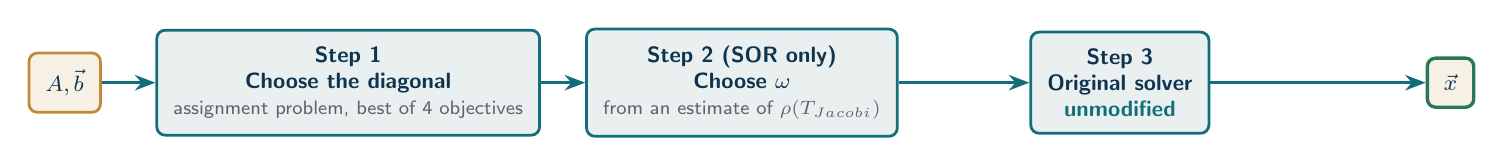
\begin{tikzpicture}
    \node[data] (in) at (0,0) {$A, \vec{b}$};
    \node[stage] (s1) at (3.6,0) {Step 1\\Choose the diagonal\subtag{assignment problem, best of 4 objectives}};
    \node[stage] (s2) at (8.6,0) {Step 2 (SOR only)\\Choose $\omega$\subtag{from an estimate of $\rho(T_{Jacobi})$}};
    \node[stage] (s3) at (13.4,0) {Step 3\\Original solver\\\emph{unmodified}};
    \node[outbox] (out) at (17.6,0) {$\vec{x}$};
    \draw[fl] (in) -- (s1);
    \draw[fl] (s1) -- (s2);
    \draw[fl] (s2) -- (s3);
    \draw[fl] (s3) -- (out);
  \end{tikzpicture}}
  \vspace{0.9em}
  \small
  \begin{itemize}\setlength\itemsep{0.35em}
    \item Every arm is measured \emph{separately} as well as \emph{together}.
      ``The pipeline helps'' is not a result; \emph{which step} helps, and by how
      much, is.
    \item Steps 1 and 2 never touch the solver itself. $A'\vec{x}=\vec{b}'$ solves
      the original system directly: nothing needs to be undone.
    \item \textbf{\color{LSteal}All seven arms have now run}, across all 927 matrices,
      413.6 minutes, no hang. What that run found is on the next two slides.
  \end{itemize}
\end{frame}

\begin{frame}{Milestone 10 (continued): SOR Through Both Steps}
  \begin{center}
  \slidefig[0.6]{24_sor_full_pipeline.png}
  \end{center}
  \vspace{0.2em}
  \footnotesize\color{LSgray}\centering
  Step 2 adds 24 on top of step 1, a 75\% increase over the as-given baseline. Not
  loss-free: relative to step 1 alone it gains 36 and loses 12, because choosing
  $\omega$ per matrix has no ``do nothing'' fallback the way step 1 does.
\end{frame}

\begin{frame}{Milestone 10 (continued): Reordering in Front of ILU, Whole Corpus}
  \begin{center}
  \slidefig[0.86]{25_ilu_full_corpus.png}
  \end{center}
  \vspace{0.2em}
  \footnotesize\color{LSgray}\centering
  The 166-matrix hole (Milestone 8) could only show gains, since its baseline was zero.
  Across all 927, ILU-BiCGSTAB and ILU-Krylov both move on identical sets: 30 gained,
  12 lost, net +18. Changing the diagonal changes what ILU factors against.
\end{frame}

%=============================================================================
\dividerframe{PART 6}{Honest Limits}{What we do and do not claim, stated plainly}
%=============================================================================

\begin{frame}{What We Do Not Claim}
  \small
  \begin{itemize}\setlength\itemsep{0.55em}
    \item \textbf{We do not claim to have beaten MC64.} Against MC64 alone our
      portfolio is worth \textbf{+2} systems solved. The reordering \emph{idea}
      carries 199; our own objective is a small part of it.
    \item \textbf{We do not claim min-sum is a second, independent idea.} It is
      MC64, proved algebraically and verified on 193 matrices.
    \item \textbf{We do not claim the diagonal-dominance guarantee is reachable
      here.} 43 matrices already have it; zero more can be reached by any row
      permutation on this corpus.
    \item \textbf{We do not claim a new iterative method.} This is a preprocessing
      pipeline in front of solvers that are otherwise completely unmodified.
    \item \textbf{We do not claim the full pipeline is loss-free.} Step 2 gains 36 and
      loses 12 on top of step 1 for SOR; reordering in front of ILU gains 30 and loses
      12 across the whole corpus. Only step 1 alone is guaranteed never to lose.
  \end{itemize}
  \vspace{0.5em}
  \colorbox{LSlightgold}{\parbox{0.95\linewidth}{\centering\footnotesize
  What we do claim: a diagnosed cause, a principled objective with a proof behind
  it, and a measured, honest gain. That is what the story in Part 5 is built on.}}
\end{frame}

%=============================================================================
\dividerframe{PART 7}{Where Things Stand}{Everything planned has run. What comes next}
%=============================================================================

\begin{frame}{Status Right Now}
  \small
  \renewcommand{\arraystretch}{1.02}
  \begin{center}
  \begin{tabular}{@{}p{6.7cm}p{4.0cm}@{}}
    \toprule
    \hdrow \hdtxt{Piece} & \hdtxt{Status}\\
    \midrule
    16-method main sweep, 927 matrices & \gd{done}\\
    \rowcolor{LSlight}
    Spectral analysis (theory vs.\ reality) & \gd{done}\\
    Refinement study & \gd{done}\\
    \rowcolor{LSlight}
    Reordering study (stationary methods) & \gd{done}\\
    ILU-hole diagnosis (166 matrices) & \gd{done}\\
    \rowcolor{LSlight}
    Adaptive-omega probe (400 matrices) & \gd{done}\\
    Full 7-arm pipeline, whole corpus & \gd{done}\\
    \bottomrule
  \end{tabular}
  \end{center}
  \vspace{0.1em}
  \colorbox{LSlightgold}{\parbox{0.96\linewidth}{\centering\footnotesize
  \textbf{Every planned run has finished. Nothing in this project is still running.}}}
  \vspace{0.1em}
  \footnotesize\color{LSgray}
  353 further SuiteSparse matrices have been downloaded into a separate folder for
  a possible future, larger run. They are deliberately not mixed into the 927 this
  project's numbers are measured on.
\end{frame}

\begin{frame}{Eight Mistakes We Made, and Fixed}
  \scriptsize
  \begin{enumerate}\setlength\itemsep{0.28em}
    \item Trusted a solver's own success flag (57 false successes, residual $10^{12}$).
    \item Divided success rates by the whole corpus instead of by applicability.
    \item Gave iterative refinement to one method only.
    \item Gauss-Seidel and SOR re-factored inside the loop, inflating runtime 11--14x.
    \item A divergence guard that killed genuine, slow-to-turn convergences.
    \item Two copies of the library quietly drifted apart.
    \item Downloaded files were never checked against their own declared size.
    \item Trusted two scipy routines without testing them on real data first.
  \end{enumerate}
  \vspace{0.4em}
  \footnotesize\color{LSgray}\centering
  Full detail on every one of these, with the number each fix changed, is in
  \texttt{Presentation/explaination.md} and \texttt{docs/GUIDE.md}.
\end{frame}

\begin{frame}[plain]
  \begin{tikzpicture}[remember picture,overlay]
    \fill[LSnavy] (current page.north west) rectangle (current page.south east);
  \end{tikzpicture}
  \vspace{2.6cm}
  \begin{center}
  {\color{white}\fontsize{30}{34}\selectfont\bfseries Thank You}\\[0.7em]
  {\color{LSgold}\large Questions?}\\[1.3em]
  {\color{LSlight}\normalsize SolveBench \;$\cdot$\; CSE 402, Section A2}\\[0.3em]
  {\color{LSlight}\footnotesize \memberOne\ $\cdot$ \memberTwo\ $\cdot$ \memberThree\ $\cdot$ \memberFour\ $\cdot$ \memberFive}
  \end{center}
\end{frame}

\end{document}
